\documentclass{article}

\usepackage[utf8]{inputenc}
\usepackage[T1]{fontenc}
\usepackage{polski}

\usepackage{lastpage}
\usepackage{graphicx} 

\usepackage[colorlinks = true,
            linkcolor = black,
            urlcolor  = blue,
            citecolor = blue,
            anchorcolor = blue]{hyperref}

\usepackage{caption}

\captionsetup[figure]{name={Rysunek}}
\hoffset=-1.0cm

\usepackage{fancyhdr}
\pagestyle{fancy}
\fancyhf{}
\rfoot{Strona \thepage \hspace{1pt} z \pageref{LastPage}}

\title{Symulacja pracy z Tablicą Kanban - aplikacja webowa - Sprawozdanie końcowe}
\author{}
\date{}

\begin{document}
\maketitle

\begin{flushright}
\par
\vfill
\par
Wykonał: Bartosz Zakrzewski

Data: 31.05.2021

\end{flushright}
\thispagestyle{empty}

\tableofcontents

\section{Podsumowanie projektu}

\subsection{Tematyka}
Projekt miał na celu stworzenie aplikacji webowej, która pozwalałaby na symulację pracy z tablicą Kanban. W takiej symulacji kilku członków zespołu developerskiego pracuje nad projektem, w którym występują różne rodzaje zadań.

\subsection{Podsumowanie}

\begin{itemize}
    \item Udało się wykonać zadaną funkcjonalność.
    
    \item Czas trwania projektu to około 2 miesiące (Kwiecień - Czerwiec 2021).
    
    \item Aplikacja webowa została stworzona za pomocą frameworka JavaScript Vue.js (i technologii HTML i CSS).

    \item Aplikacja jest aplikacją Frontend, co oznacza, że nie ma rejestracji, ani możliwości zapisania wyników pracy (Użytkownik może dokonać symulacji i wynik zapisać np. za pomocą zrzutu ekranu).
    
    \item Strona została zhostowana za pomocą Github Pages:
    
    \href{https://zakrzewskib.github.io/KanbanWorkflowSimulation/}{https://zakrzewskib.github.io/KanbanWorkflowSimulation/}.
    
\end{itemize}


\section{Wykonana funkcjonalność}

\subsection{Zakres pracy}
\begin{itemize}
    \item Definiowanie limitów ilości zadań w poszczególnej kolumnie;
    \item Oznaczanie wykonanej pracy - wypełnianie progresu wewnątrz danego zadania/taska;
    \item Mechanizm rzucania kostką 1-5 - jest to generowanie produktywności danego dnia dla danej osoby;
    \item Generowanie blokerów - daje znać użytkownikowi, że z zadaniem są trudności, Blokera da się usunąć np. wykorzystując punkty progresu;
    \item Przypisywanie osoby do zadania (oznaczenie kolorystyczne);
    \item 3 rodzaje taska: Zwykły, Urgent, Fixed Date (nazwa i np. dodatkowo kolorystyka);
    \item Zadanie ma pole do wpisania dnia początkowego i końcowego;
    \item Ustalanie prawdopodobieństwa generowania blokerów;
    \item Symulacja jest oparta na historiach opisujących kolejne dni pracy;
\end{itemize}

\clearpage

\subsection{Wygląd aplikacji}

    \begin{figure} [hbt!]
        \centering
        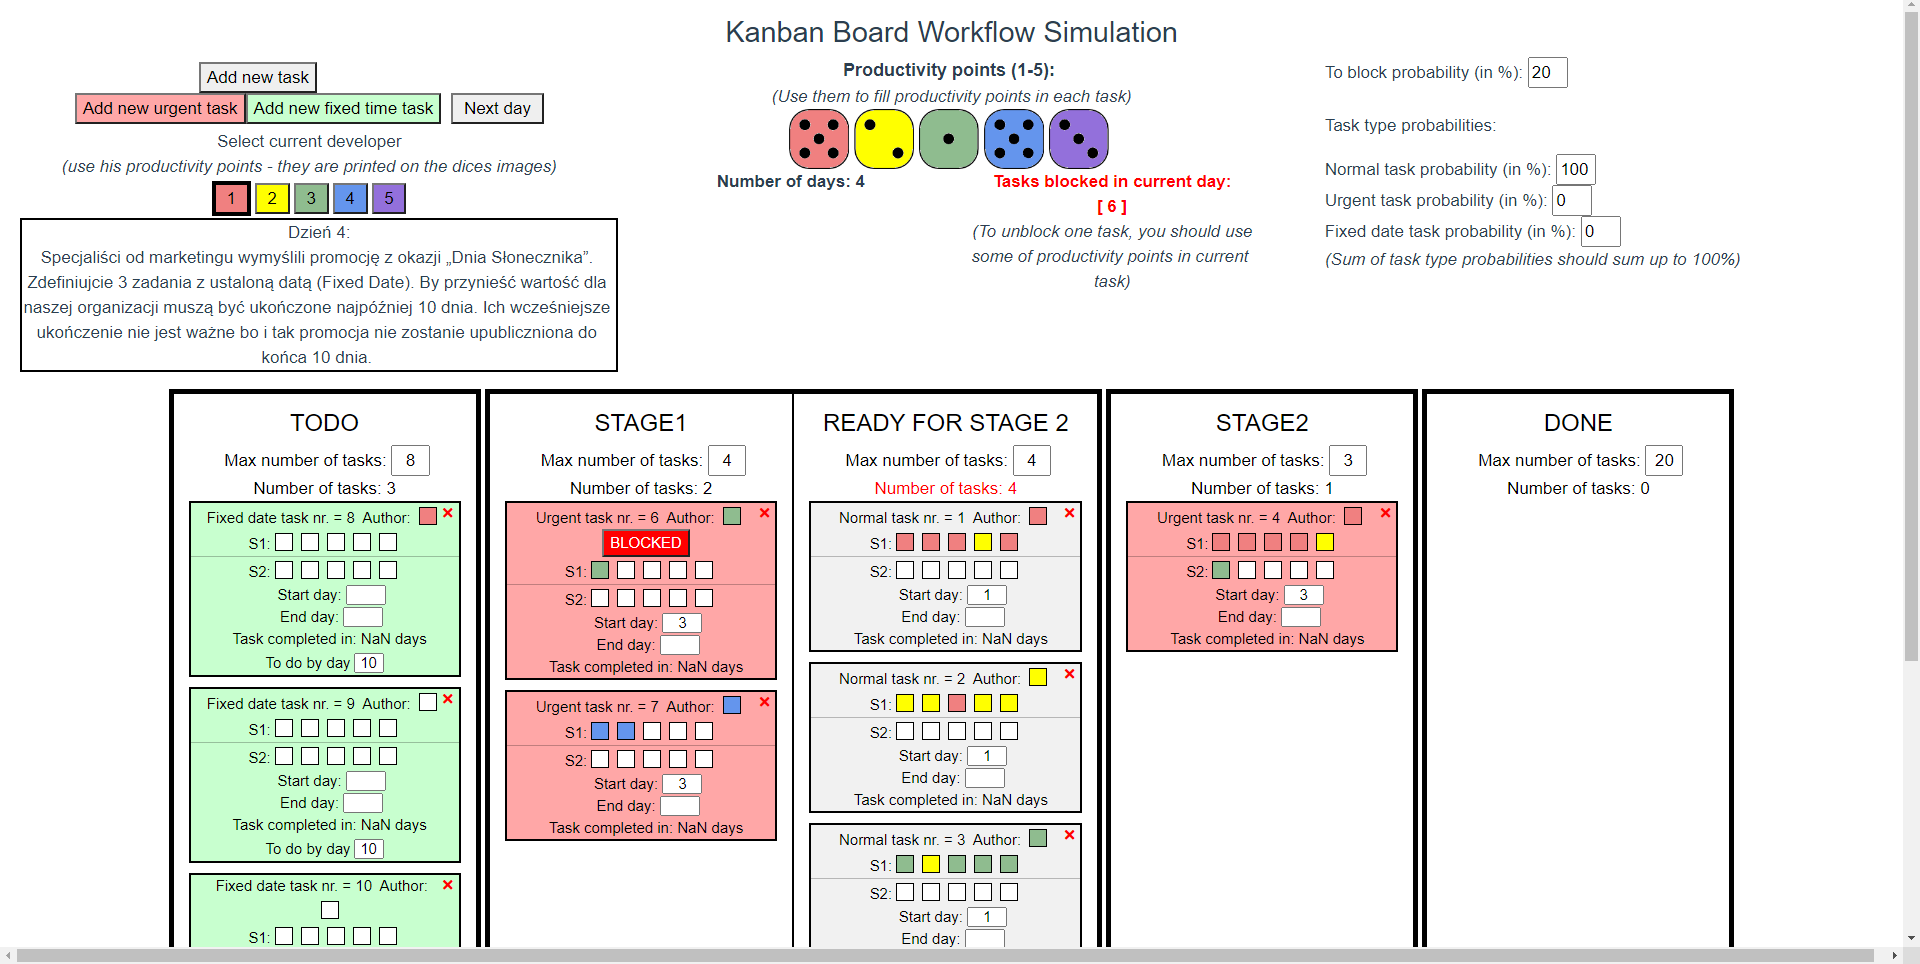
\includegraphics[width=16cm]{img/wygląd strony.PNG}
        \captionof{figure}{Wygląd aplikacji}
    \end{figure}


\subsection{Poszczególne elementy aplikacji}

\subsection{Kolumny}
\begin{itemize}
    \item Jeżeli zadania są w kolumnach TODO lub READY FOR STAGE 2 lub DONE nie mogą być zablokowane.
    \item W każdej kolumnie jest określona poglądowa maksymalna ilość zadań.
    \item Zadania można przenosić między kolumnami.
\end{itemize}

\subsection{Zadania}
\begin{itemize}
    \item Są trzy rodzaje zadań: Normal, Urgent i Fixed Date.
    \item Poszczególne rodzaje zadań są oznaczone kolorami.
    \item Każde zadanie ma:
    \begin{itemize}
        \item autora,
        \item punkty progresu,
        \item dzień rozpoczęcia i zakończenia,
        \item czas trwania wykonywania zadania,
        \item przycisk usunięcia zadania ('x').
    \end{itemize}
    \item Dodatkowo zadanie FixedDate ma określone do jakiego dnia trzeba je ukończyć.
\end{itemize}

\subsection{Dodatkowe}
\begin{itemize}
    \item Trzy przyciski dodawania nowego zadania.
    \item Wybór którego developera punkty zużywamy.
    \item Kostki do gry pokazujące produktywność każdego z developerów.
    \item Przycisk rozpoczynający nowy dzień - powoduje on losowanie nowych punktów produktywności, blokowanie losowo zadań i zwiększanie się liczby dni symulacji.
    \item Informacja jakie zadania zostały zablokowane danego dnia.
    \item Prawdopodobieństwa zablokowania danego zadania i jaki task zostanie stworzony po naciśnięciu przycisku 'Add new task' (można je zmienić).
    \item Historie opisujące kolejne dni. Po 10 dniach symulacji nie ma już więcej narracji, aczkolwiek użytkownik może nadal prowadzić symulację. 
\end{itemize}

\section{Narzędzia}

\subsection{Środowisko pracy}
\begin{itemize}
    \item IDE - Visual Studio Code 1.56.2
    \item System kontroli wersji git 2.29.2.windows.3.
    \item Repozytorium zdalne na stronie github:
    
    \href{https://github.com/zakrzewskib/KanbanWorkflowSimulation}{https://github.com/zakrzewskib/KanbanWorkflowSimulation}
    
    \item Strona została zhostowana za pomocą Github Pages:
    
    \href{https://zakrzewskib.github.io/KanbanWorkflowSimulation/}{https://zakrzewskib.github.io/KanbanWorkflowSimulation/}.
    
\end{itemize}

\clearpage

\subsection{Struktura projektu}

\subsection{Komponenty}

Aplikacja składa się z komponentów:

\begin{figure} [hbt!]
    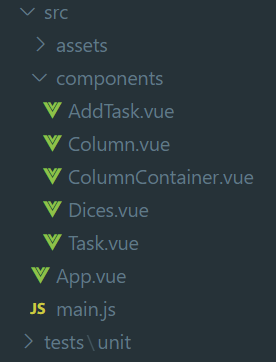
\includegraphics[width=5cm,center]{img/komponenty.PNG}
    \captionof{figure}{Komponenty projektu}
\end{figure}

Aplikacja nie ma wielu komponentów i dodatkowo główny komponent ma dużą liczbę linii - było to prostsze do implementacji w technologii Vue.js.

\subsection{Pakiety}
    npmPackages:
\begin{itemize}
    \item @vue/babel-helper-vue-jsx-merge-props:  1.2.1
    \item @vue/babel-helper-vue-transform-on:  1.0.2
    \item @vue/babel-plugin-jsx:  1.0.4
    \item @vue/babel-plugin-transform-vue-jsx:  1.2.1
    \item @vue/babel-preset-app:  4.5.12
    \item @vue/babel-preset-jsx:  1.2.4
    \item @vue/babel-sugar-composition-api-inject-h:  1.2.1
    \item @vue/babel-sugar-composition-api-render-instance:  1.2.4
    \item @vue/babel-sugar-functional-vue:  1.2.2
    \item @vue/babel-sugar-inject-h:  1.2.2
    \item @vue/babel-sugar-v-model:  1.2.3
    \item @vue/babel-sugar-v-on:  1.2.3
    \item @vue/cli-overlay:  4.5.13
    \item @vue/cli-plugin-babel: ~4.5.0 => 4.5.12
    \item @vue/cli-plugin-eslint: ~4.5.0 => 4.5.12
    \item @vue/cli-plugin-router:  4.5.13
    \item @vue/cli-plugin-unit-jest: ~4.5.0 => 4.5.13
    \item @vue/cli-plugin-vuex:  4.5.13
    \item @vue/cli-service: \^{}4.5.13 => 4.5.13
    \item @vue/cli-shared-utils:  4.5.13 (4.5.12)
    \item @vue/component-compiler-utils:  3.2.0
    \item @vue/preload-webpack-plugin:  1.1.2
    \item @vue/test-utils: \^{}1.0.3 => 1.2.0
    \item @vue/web-component-wrapper:  1.3.0
    \item bootstrap-vue: \^{}2.21.2 => 2.21.2
    \item eslint-plugin-vue: \^{}6.2.2 => 6.2.2
    \item jest-serializer-vue:  2.0.2
    \item portal-vue:  2.1.7
    \item vue: \^{}2.6.12 => 2.6.12
    \item vue-eslint-parser:  7.6.0
    \item vue-functional-data-merge:  3.1.0
    \item vue-hot-reload-api:  2.3.4
    \item vue-jest:  3.0.7
    \item vue-loader:  15.9.6 (16.2.0)
    \item vue-style-loader:  4.1.3
    \item vue-template-compiler: \^{}2.6.11 => 2.6.12
    \item vue-template-es2015-compiler:  1.9.1
\end{itemize}

\section{Uruchomienie kodu}
Jeżeli pobierzemy kod z repozytorium na Githubie (i np. dodamy jakąś funkcjonalność) wynik pracy można zobaczyć za pomocą yarn - menadżera pakietów:
\begin{enumerate}
    \item yarn install - instalacja yarn'a;
    \item yarn serve - aby zobaczyć poglądowo naszą aplikację;
\end{enumerate}

Można to także wykonać za pomocą innego menadżera pakietów - npm:
\begin{enumerate}
    \item npm install - instalacja npm;
    \item npm run serve - zobaczenie aplikacji;
\end{enumerate}

Aby zbudować projekt i zhostować aplikację webową należy:
\begin{enumerate}
    \item yarn build - utworzy nam się folder dist; (lub npm run build)
    \item folder dist jest gotowy na wdrożenie;
    \item następnie należy postępować zgodnie z instrukcją na \\ \href{https://cli.vuejs.org/guide/deployment.html#github-pages}{https://cli.vuejs.org/guide/deployment.html\#github-pages}, aby skorzystać z serwisu Github Pages.
    W repozytorium pliki potrzebne do użycia Github pages to deploy.sh i vue.config.js.
\end{enumerate}

\section{Źródła}
\begin{itemize}
    \item Pomysł na aplikację: https://www.okaloa.com/.
    \item Zakres projektu został zaprezentowany przez opiekuna projektu: mgr. inż. Krzysztofa Marka.
    \item Framework Vue.js: https://vuejs.org/
\end{itemize}

\end{document}